\documentclass{article}

\usepackage{graphicx}
\usepackage{setspace}

\title{ECE 210 - Combinational Logic Design \\
    Lab 2}
\date{2018-10-24}
\author{David Lenfesty \and Radomir Wasowski}

\setcounter{tocdepth}{2} % Show subsections

\begin{document}

    \pagenumbering{gobble}
    \maketitle
    \newpage

    \doublespacing
    \tableofcontents
    \newpage


    \singlespacing
    \pagenumbering{arabic}

    \section{Abstract}

    This lab report is about FPGAs

    We do cool things with them.
    BLAHLADUWBDAWDWAUDKBB


    Howiandwan?


    \section{Introduction}
    This lab report will be cool because it's using LaTeX.

    \section{Design Section}
    stuff

    \paragraph{Part 1}

    \paragraph{Part 2}

    \section{Procedure}
    We typed things

    \paragraph{Part 1}

    Simu

    \paragraph{Part 2}


    \section{Results}
    Lights flashed

    \begin{figure}[b!]
        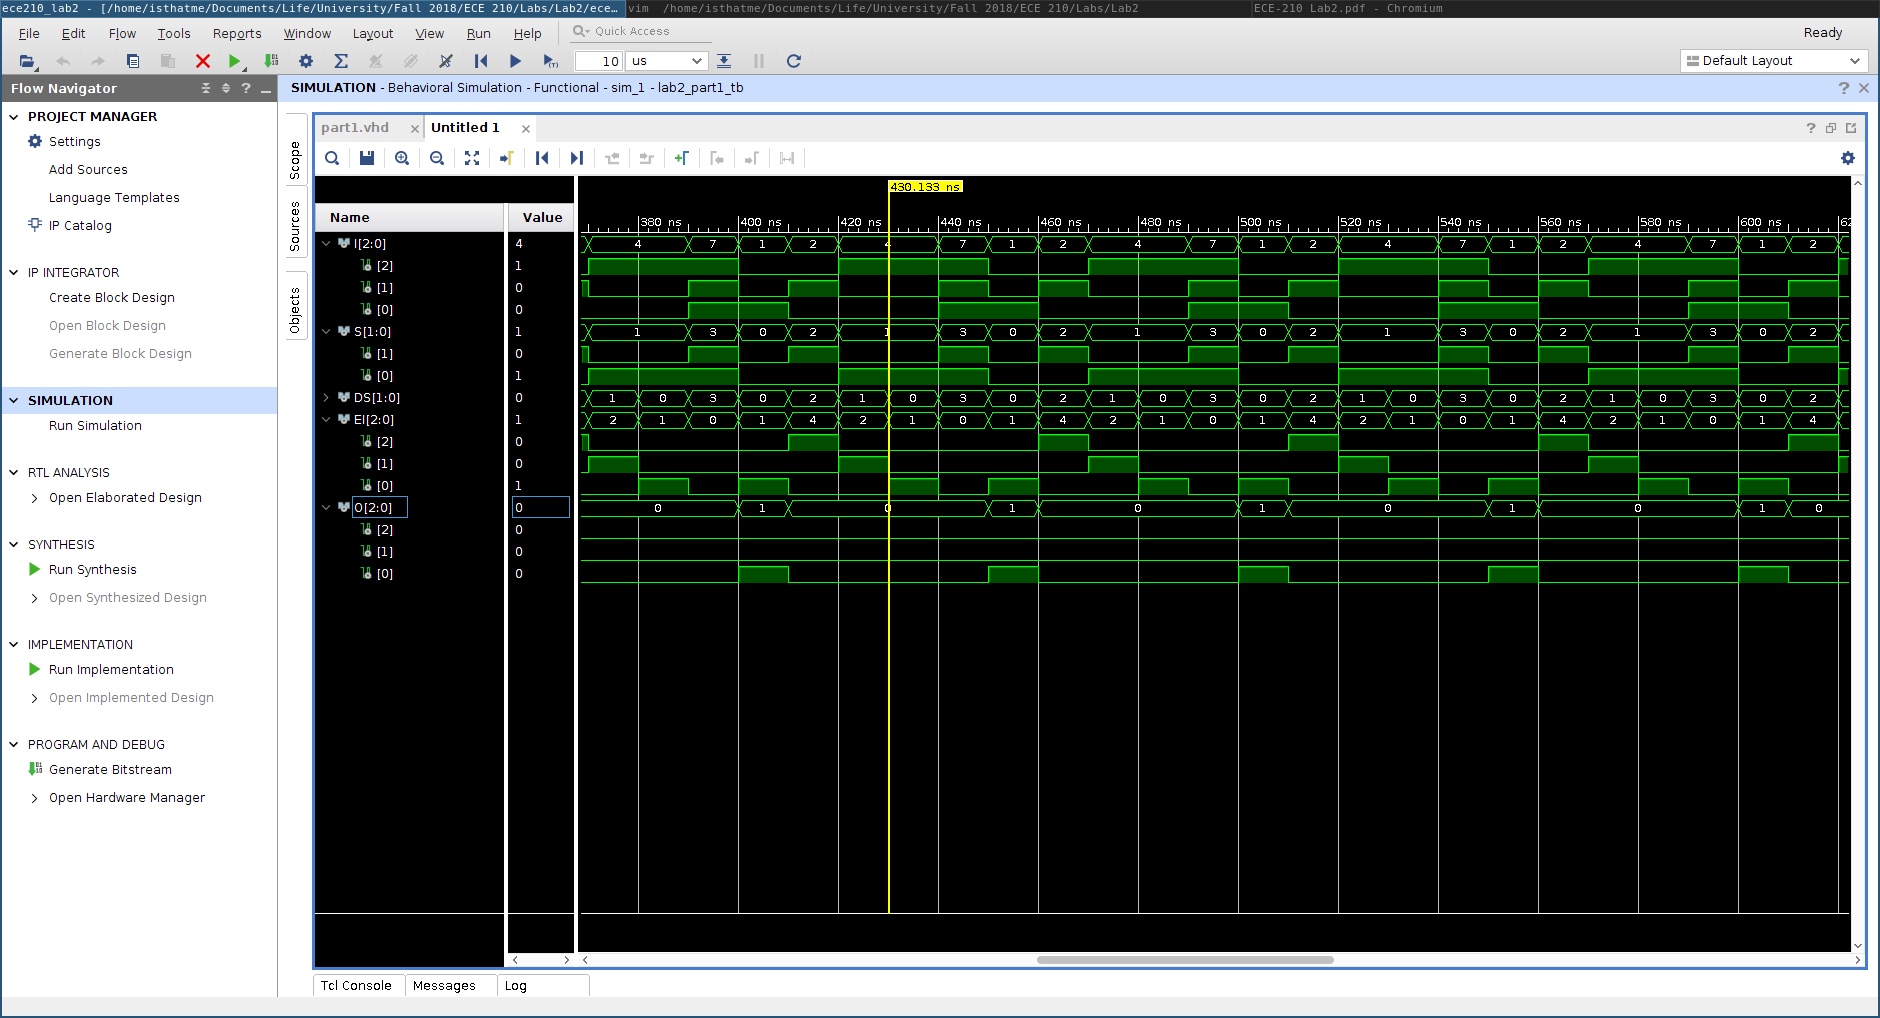
\includegraphics[width=\linewidth]{MUX_DEMUX.png}
        \caption{Part 1 Simulation.}
        \label{fig:part1_sim}
    \end{figure}

    \paragraph{Part 1}


    \paragraph{Part 2}


    \section{Discussion}
    Dogs are better than cats.
    End of discussion

    \section{Conclusion}
    Blinkies are cool.


\end{document}

